\documentclass[border=12pt]{standalone}
\usepackage{tikz}
\usetikzlibrary{arrows.meta, positioning, calc, fit, backgrounds}
\usepackage{amsmath, amssymb}

% ── Palette ────────────────────────────────────────────────────────────────
\definecolor{gnnblue}{RGB}{70,130,190}
\definecolor{gnnfill}{RGB}{210,228,248}
\definecolor{bpgreen}{RGB}{60,155,90}
\definecolor{bpfill}{RGB}{210,240,215}
\definecolor{filmorange}{RGB}{210,120,40}
\definecolor{fillfill}{RGB}{252,235,205}
\definecolor{iogray}{RGB}{100,100,100}
\definecolor{iofill}{RGB}{235,235,235}
\definecolor{plusgray}{RGB}{80,80,80}

\begin{document}
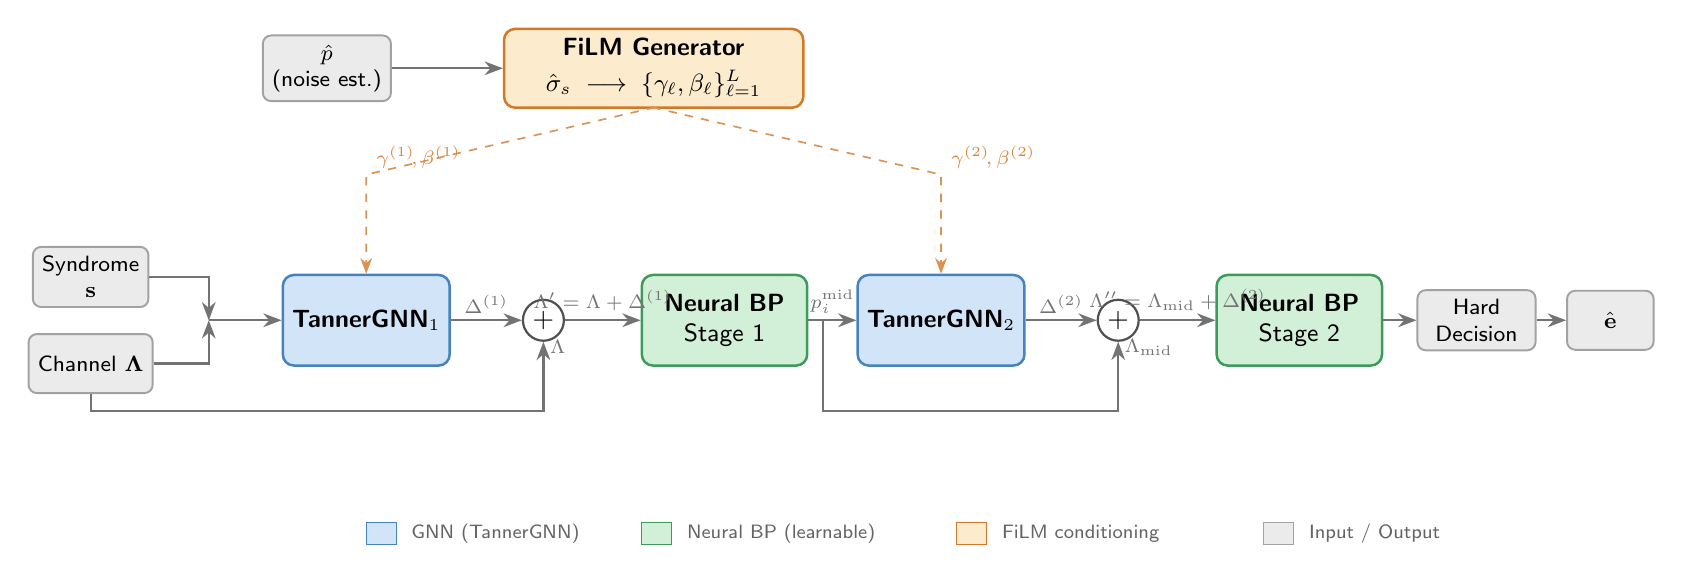
\begin{tikzpicture}[
    >=Stealth,
    font=\sffamily\small,
    % ── Node styles ──────────────────────────────────────────────────────
    gnn/.style={
        rectangle, draw=gnnblue, fill=gnnfill, line width=0.9pt,
        rounded corners=4pt, minimum width=2.1cm, minimum height=1.15cm,
        align=center, font=\sffamily\small
    },
    bp/.style={
        rectangle, draw=bpgreen, fill=bpfill, line width=0.9pt,
        rounded corners=4pt, minimum width=2.1cm, minimum height=1.15cm,
        align=center, font=\sffamily\small
    },
    film/.style={
        rectangle, draw=filmorange, fill=fillfill, line width=0.9pt,
        rounded corners=4pt, minimum width=3.8cm, minimum height=1.0cm,
        align=center, font=\sffamily\small
    },
    io/.style={
        rectangle, draw=iogray!60, fill=iofill, line width=0.7pt,
        rounded corners=3pt, minimum width=1.1cm, minimum height=0.75cm,
        align=center, font=\sffamily\footnotesize
    },
    plus/.style={
        circle, draw=plusgray, fill=white, line width=0.8pt,
        minimum size=0.52cm, inner sep=0pt,
        font=\sffamily\normalsize
    },
    hard/.style={
        rectangle, draw=iogray!60, fill=iofill, line width=0.7pt,
        rounded corners=3pt, minimum width=1.5cm, minimum height=0.75cm,
        align=center, font=\sffamily\footnotesize
    },
    % ── Arrow styles ─────────────────────────────────────────────────────
    mainarr/.style={->, thick, black!55},
    filmarr/.style={->, semithick, filmorange!80, dashed},
    labelnode/.style={font=\sffamily\scriptsize, inner sep=2pt}
]

% ════════════════════════════════════════════════════════════════════════════
%  ROW POSITIONS
%    film_y  = 5.2   (FiLM generator row)
%    pipe_y  = 2.0   (main pipeline row)
%    gamma_y = 3.7   (γ,β label clearance row — between film and pipe)
% ════════════════════════════════════════════════════════════════════════════

% ── Input nodes ─────────────────────────────────────────────────────────────
\node[io] (syn)  at (-3.5, 2.55) {Syndrome\\$\mathbf{s}$};
\node[io] (llr)  at (-3.5, 1.45) {Channel $\boldsymbol{\Lambda}$};

% ── Merge of syndrome + LLR into first GNN ──────────────────────────────────
% (a small invisible join point)
\coordinate (join) at (-2.0, 2.0);

% ── TannerGNN₁ ──────────────────────────────────────────────────────────────
\node[gnn] (gnn1) at (0.0, 2.0) {\textbf{TannerGNN}$_1$};

% ── Adder 1 ─────────────────────────────────────────────────────────────────
\node[plus] (add1) at (2.25, 2.0) {$+$};

% ── Neural BP Stage 1 ───────────────────────────────────────────────────────
\node[bp]  (bp1)  at (4.55, 2.0) {\textbf{Neural BP}\\Stage 1};

% ── p_i^{mid} label sits on the arrow between BP1 and GNN2
%    (placed at mid arrow, above the line)

% ── TannerGNN₂ ──────────────────────────────────────────────────────────────
\node[gnn] (gnn2) at (7.3, 2.0) {\textbf{TannerGNN}$_2$};

% ── Adder 2 ─────────────────────────────────────────────────────────────────
\node[plus] (add2) at (9.55, 2.0) {$+$};

% ── Neural BP Stage 2 ───────────────────────────────────────────────────────
\node[bp]  (bp2)  at (11.85, 2.0) {\textbf{Neural BP}\\Stage 2};

% ── Hard Decision ───────────────────────────────────────────────────────────
\node[hard] (hd) at (14.1, 2.0) {Hard\\Decision};

% ── Output ──────────────────────────────────────────────────────────────────
\node[io]  (out) at (15.8, 2.0) {$\hat{\mathbf{e}}$};

% ── FiLM Generator (top row, well above pipeline) ───────────────────────────
\node[film] (film) at (3.65, 5.2)
    {\textbf{FiLM Generator}\\[2pt]
     $\hat{\sigma}_s \;\longrightarrow\; \{\gamma_\ell,\beta_\ell\}_{\ell=1}^{L}$};

% Noise estimator feeding FiLM
\node[io] (noiseest) at (-0.5, 5.2) {$\hat{p}$\\(noise est.)};
\draw[mainarr] (noiseest) -- (film.west);

% ════════════════════════════════════════════════════════════════════════════
%  FiLM → GNN branches
%  Route: film.south → down to γ,β label clearance height → then to GNN tops
%  Labels placed at the bend point, well clear of both the film box and GNNs
% ════════════════════════════════════════════════════════════════════════════

% Branch point on film bottom
\coordinate (filmbottom) at (3.65, 4.7);

% Left FiLM branch: goes to gnn1 top
\coordinate (filmL_bend) at (0.0, 3.85);
\draw[filmarr]
    (film.south) -- (filmbottom)
    -- (filmL_bend) -- (gnn1.north);
\node[labelnode, filmorange!90, above right] at ($(filmL_bend)+(0.05,0)$)
    {$\gamma^{(1)}\!,\beta^{(1)}$};

% Right FiLM branch: goes to gnn2 top
\coordinate (filmR_bend) at (7.3, 3.85);
\draw[filmarr]
    (film.south) -- (filmbottom)
    -- (filmR_bend) -- (gnn2.north);
\node[labelnode, filmorange!90, above right] at ($(filmR_bend)+(0.05,0)$)
    {$\gamma^{(2)}\!,\beta^{(2)}$};

% ════════════════════════════════════════════════════════════════════════════
%  Main pipeline arrows
% ════════════════════════════════════════════════════════════════════════════

% Syndrome + channel → join → gnn1
\draw[mainarr] (syn.east)  -| (join);
\draw[mainarr] (llr.east)  -| (join);
\draw[mainarr] (join) -- (gnn1.west);

% GNN1 → adder1: label Δ^(1) above arrow, away from node edges
\draw[mainarr] (gnn1.east) -- (add1.west)
    node[labelnode, above, midway] {$\Delta^{(1)}$};

% Channel passthrough to adder1 (Λ enters from below)
\coordinate (llr_to_add1) at (2.25, 0.85);
\draw[mainarr] (llr.south) |- (llr_to_add1) -- (add1.south)
    node[labelnode, right, pos=0.92] {$\Lambda$};

% adder1 → bp1
\draw[mainarr] (add1.east) -- (bp1.west)
    node[labelnode, above, midway, yshift=1pt]
    {$\Lambda' = \Lambda + \Delta^{(1)}$};

% bp1 → gnn2: label p_i^{mid} above arrow
\draw[mainarr] (bp1.east) -- (gnn2.west)
    node[labelnode, above, midway] {$p_i^{\mathrm{mid}}$};

% GNN2 → adder2: label Δ^(2) above arrow
\draw[mainarr] (gnn2.east) -- (add2.west)
    node[labelnode, above, midway] {$\Delta^{(2)}$};

% Mid-LLR passthrough to adder2 (from bp1 output, routed below)
\coordinate (midllr_src) at (5.8, 2.0);
\coordinate (midllr_low) at (5.8, 0.85);
\coordinate (add2_below) at (9.55, 0.85);
\draw[mainarr] (midllr_src) |- (midllr_low) -- (add2_below) -- (add2.south)
    node[labelnode, right, pos=0.92] {$\Lambda_{\mathrm{mid}}$};

% adder2 → bp2
\draw[mainarr] (add2.east) -- (bp2.west)
    node[labelnode, above, midway, yshift=1pt]
    {$\Lambda'' = \Lambda_{\mathrm{mid}} + \Delta^{(2)}$};

% bp2 → hard decision → output
\draw[mainarr] (bp2.east) -- (hd.west);
\draw[mainarr] (hd.east)  -- (out.west);

% ════════════════════════════════════════════════════════════════════════════
%  Legend  (bottom strip, well below pipeline)
% ════════════════════════════════════════════════════════════════════════════
\begin{scope}[shift={(0.0, -0.85)}]

\fill[gnnfill]   (0.0, 0) rectangle (0.38, 0.28);
\draw[gnnblue]   (0.0, 0) rectangle (0.38, 0.28);
\node[anchor=west, font=\sffamily\scriptsize, iogray]
    at (0.45, 0.14) {GNN (TannerGNN)};

\fill[bpfill]    (3.5, 0) rectangle (3.88, 0.28);
\draw[bpgreen]   (3.5, 0) rectangle (3.88, 0.28);
\node[anchor=west, font=\sffamily\scriptsize, iogray]
    at (3.95, 0.14) {Neural BP (learnable)};

\fill[fillfill]  (7.5, 0) rectangle (7.88, 0.28);
\draw[filmorange](7.5, 0) rectangle (7.88, 0.28);
\node[anchor=west, font=\sffamily\scriptsize, iogray]
    at (7.95, 0.14) {FiLM conditioning};

\fill[iofill]    (11.4, 0) rectangle (11.78, 0.28);
\draw[iogray!60] (11.4, 0) rectangle (11.78, 0.28);
\node[anchor=west, font=\sffamily\scriptsize, iogray]
    at (11.85, 0.14) {Input / Output};

\end{scope}

\end{tikzpicture}
\end{document}
